% !TeX TS-program = txs:///duck
\documentclass{standalone}
\usepackage{tikzducks}

\definecolor{skin}{RGB}{255,209,181}
\definecolor{lblue}{RGB}{176,172,188}
\definecolor{lbrown}{RGB}{236,213,163}
\definecolor{dbrown}{RGB}{176,134,95}
\definecolor{billcol}{RGB}{230,132,82}

\begin{document}
	
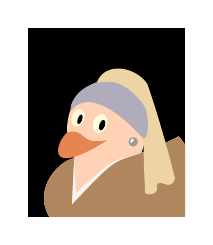
\begin{tikzpicture}

  \fill[black] (-0.1,0.4) rectangle (1.9,2.8); 

  \clip (-0.1,0.4) rectangle (1.9,2.8); 


	\duck[
		body=skin, 
		jacket=dbrown!10!white, 
    bill=billcol
	]
  
   \fill[dbrown]  (0.490,1.145) .. controls (0.267, 1.102) and (-0.125,0.657) .. (0.289,0.261) .. controls (0.704,-0.135) and ( 2.863,0.130) .. (1.818,1.419) .. controls (0.880, 0.946) and ( 1.240,1.378) .. (0.46,0.55) -- cycle;
  
  \begin{scope}[scale=0.12,xshift=-1.3cm,yshift=3.8cm]
    \fill[lbrown] (7.7941,13.7509) .. controls (10.8320,13.4186) and (11.7764,12.3930) .. (12.6964,10.9465) .. controls (12.6964,10.9465) and (12.6769,5.6002) .. (12.9122,2.0156) .. controls (13.2041,1.7780) and (13.7523,1.8952) .. (14.0339,2.1451) .. controls (14.2660,2.3512) and (13.9970,2.8707) .. (14.2496,3.0512) .. controls (14.6140,3.3115) and (15.1783,2.7387) .. (15.5871,2.9217) .. controls (15.8312,3.0309) and (16.0169,3.3052) .. (16.0616,3.5688) .. controls (16.0616,3.5688) and (14.7664,8.8740) .. (13.1278,13.5783) .. controls (11.9515,15.3829) and (8.6715,16.0161) .. (7.7941,13.7509) -- cycle;
    \fill[lblue] (4.9884,10.6533) .. controls (7.4488,14.0291) and (12.6964,7.7969) .. (12.6964,7.7969) .. controls (13.4861,7.8582) and (13.1708,10.7423) .. (12.8259,11.2053) .. controls (10.9927,13.8335) and (9.2448,13.7940) .. (9.2448,13.7940) .. controls (6.4433,14.0475) and (4.8380,11.8428) .. (4.9884,10.6533) -- cycle;
  \end{scope}
  
  \fill[gray!80!white] (1.24,1.35) circle[radius=0.06];
  \fill[white] (1.225,1.365) ellipse[x radius=0.015, y radius=0.03,rotate=-30];

  
\end{tikzpicture}

\end{document}